Use Venn diagrams to show that the associative law holds for symmetric difference; that is, for any sets $A$, $B$, and $C$, $A \triangle (B \triangle C) = (A \triangle B) \triangle C$.

\textbf{Solution:} We will tackle the first expression, piece by piece.
\begin{itemize}
    \item By the definition of the symmetric difference we can write the expressions shown above as shown below:
    \begin{align*}
        A \triangle (B \triangle C) &\equiv (A \mybackslash (B \triangle C)) \cup ((B \triangle C) \mybackslash A) \\
        &\equiv (A \mybackslash [(B \mybackslash C) \cup (C \mybackslash B)]) \cup ([(B \mybackslash C) \cup (C \mybackslash B)] \mybackslash A) \\
    \end{align*}

    We tackle the LHS of the logical sentence first, namely $A \mybackslash (B \triangle C)$. For now, we ignore $A$, in this context we know that  $B \triangle C$ is shown below:

        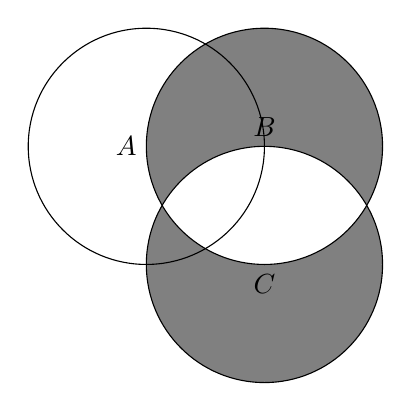
\begin{tikzpicture}
          % Define circles for A, B, and C
          \def\circleA{(0,0) circle (1.5cm)}
          \def\circleB{(1.5,0) circle (1.5cm)}
          \def\circleC{(1.5,-1.5) circle (1.5cm)}
        
          % Fill A
          \begin{scope}
            \fill[white] \circleA;
          \end{scope}
        
          % Fill B
          \begin{scope}
            \clip \circleB;
            \fill[gray] \circleB;
            \clip \circleC;
            \fill[white] \circleC;
          \end{scope}

          %Fill C
          \begin{scope}
              \clip \circleC;
              \fill[gray] \circleC;
              \clip \circleB;
              \fill[white] \circleB;
          \end{scope}
          
          % Outline the circles and label them
          \draw \circleA node [text=black, left] {$A$};
          \draw \circleB node [text=black, above] {$B$};
          \draw \circleC node [text=black, below] {$C$};
        \end{tikzpicture}

        \

    Hence, $A \mybackslash (B \triangle C)$ looks like:
    
    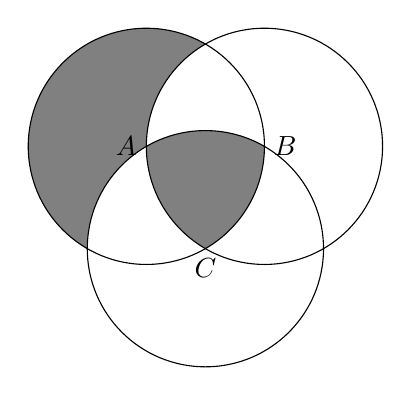
\begin{tikzpicture}
      % Define circles for A, B, and C
      \def\circleA{(0,0) circle (1.5cm)}
      \def\circleB{(1.5,0) circle (1.5cm)}
      \def\circleC{(0.75,-1.3) circle (1.5cm)}
    
      % Shade for A excluding (B \ C) and (C \ B)
      \begin{scope}
        \clip \circleA;
        \fill[gray] \circleA;
        \clip \circleB;
        \fill[white] \circleB;
      \end{scope}
      
      \begin{scope}
        \clip \circleA;
        \clip \circleC;
        \fill[white] \circleC;
      \end{scope}
    
      % Shade the intersection of A, B, and C with a different color
      \begin{scope}
        \clip \circleA;
        \clip \circleB;
        \clip \circleC;
        \fill[gray] \circleC;
      \end{scope}
      
      % Outline the circles and label them
      \draw \circleA node [text=black, left] {$A$};
      \draw \circleB node [text=black, right] {$B$};
      \draw \circleC node [text=black, below] {$C$};
    \end{tikzpicture}

    \pagebreak
    
    Meanwhile, $(B \triangle C) \mybackslash A$ looks like as shown below:

    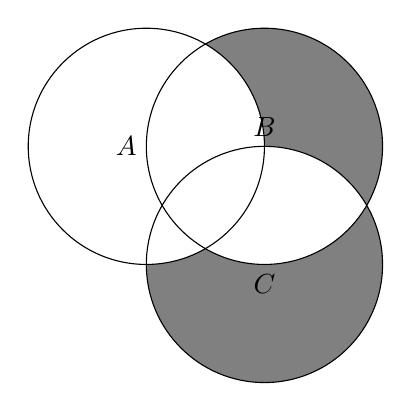
\begin{tikzpicture}
      % Define circles for A, B, and C
      \def\circleA{(0,0) circle (1.5cm)}
      \def\circleB{(1.5,0) circle (1.5cm)}
      \def\circleC{(1.5,-1.5) circle (1.5cm)}
    
      % Fill the symmetric difference of B and C
      \begin{scope}
        \clip \circleB \circleC; % Start with B and C
        \fill[gray] \circleB \circleC; % Fill B and C
        \clip \circleA; % Remove parts that overlap with A
        \fill[white] \circleA;
      \end{scope}
    
      \begin{scope}
        \clip \circleB;
        \clip \circleC;
        \fill[white] \circleC;
      \end{scope}
    
      \begin{scope}
        \clip \circleC;
        \clip \circleB;
        \fill[white] \circleB;
      \end{scope}
    
      % Outline the circles and label them
      \draw \circleA node [text=black, left] {$A$};
      \draw \circleB node [text=black, above] {$B$};
      \draw \circleC node [text=black, below] {$C$};
    \end{tikzpicture}

    Finally, we consider the union, i.e., $A \triangle (B \triangle C) \equiv (A \mybackslash (B \triangle C)) \cup ((B \triangle C) \mybackslash A)$ to get:
    
    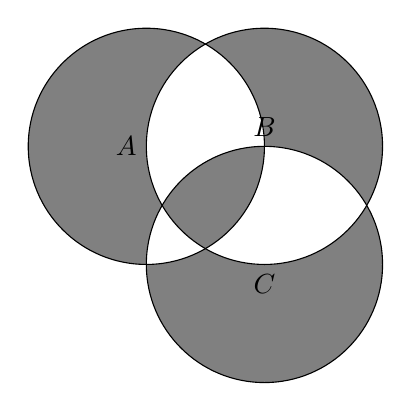
\begin{tikzpicture}
      % Define circles for A, B, and C
      \def\circleA{(0,0) circle (1.5cm)}
      \def\circleB{(1.5,0) circle (1.5cm)}
      \def\circleC{(1.5,-1.5) circle (1.5cm)}

      % Shade for A excluding (B \ C) and (C \ B)
      \begin{scope}
        \clip \circleA;
        \fill[gray] \circleA;
        \clip \circleB;
        \fill[white] \circleB;
      \end{scope}
      
      % Fill the symmetric difference of B and C
      \begin{scope}
        \clip \circleB \circleC; % Start with B and C
        \fill[gray] \circleB \circleC; % Fill B and C
        \clip \circleA; % Remove parts that overlap with A
        \fill[white] \circleA;
      \end{scope}
    
      \begin{scope}
        \clip \circleB;
        \clip \circleC;
        \fill[white] \circleC;
      \end{scope}
    
      \begin{scope}
        \clip \circleC;
        \clip \circleB;
        \fill[white] \circleB;
      \end{scope}

      % Shade the intersection of A, B, and C with a different color
      \begin{scope}
        \clip \circleA;
        \clip \circleB;
        \clip \circleC;
        \fill[gray] \circleC;
      \end{scope}
      
      % Outline the circles and label them
      \draw \circleA node [text=black, left] {$A$};
      \draw \circleB node [text=black, above] {$B$};
      \draw \circleC node [text=black, below] {$C$};
    \end{tikzpicture}
    
    \item Now, when we consider $(A \triangle B) \triangle C \equiv ((A \triangle B) \mybackslash C) \cup (C \mybackslash (A \triangle B))$, we first draw the LHS of the union below, i.e., $(A \triangle B) \mybackslash C$.

    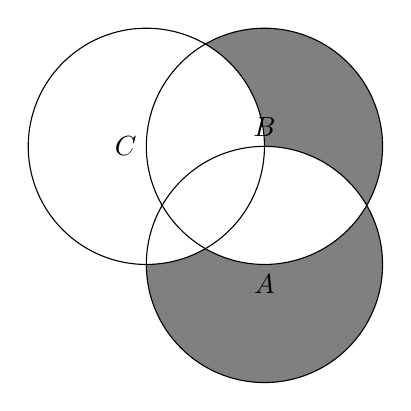
\begin{tikzpicture}
      % Define circles for A, B, and C
      \def\circleA{(0,0) circle (1.5cm)}
      \def\circleB{(1.5,0) circle (1.5cm)}
      \def\circleC{(1.5,-1.5) circle (1.5cm)}
    
      % Fill the symmetric difference of B and C
      \begin{scope}
        \clip \circleB \circleC; % Start with B and C
        \fill[gray] \circleB \circleC; % Fill B and C
        \clip \circleA; % Remove parts that overlap with A
        \fill[white] \circleA;
      \end{scope}
    
      \begin{scope}
        \clip \circleB;
        \clip \circleC;
        \fill[white] \circleC;
      \end{scope}
    
      \begin{scope}
        \clip \circleC;
        \clip \circleB;
        \fill[white] \circleB;
      \end{scope}
    
      % Outline the circles and label them
      \draw \circleA node [text=black, left] {$C$};
      \draw \circleB node [text=black, above] {$B$};
      \draw \circleC node [text=black, below] {$A$};
    \end{tikzpicture}

    \pagebreak
    Meanwhile $C \mybackslash (A \triangle B)$ looks like:

    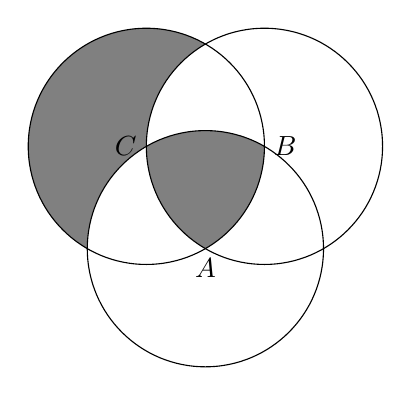
\begin{tikzpicture}
      % Define circles for A, B, and C
      \def\circleA{(0,0) circle (1.5cm)}
      \def\circleB{(1.5,0) circle (1.5cm)}
      \def\circleC{(0.75,-1.3) circle (1.5cm)}
    
      % Shade for A excluding (B \ C) and (C \ B)
      \begin{scope}
        \clip \circleA;
        \fill[gray] \circleA;
        \clip \circleB;
        \fill[white] \circleB;
      \end{scope}
      
      \begin{scope}
        \clip \circleA;
        \clip \circleC;
        \fill[white] \circleC;
      \end{scope}
    
      % Shade the intersection of A, B, and C with a different color
      \begin{scope}
        \clip \circleA;
        \clip \circleB;
        \clip \circleC;
        \fill[gray] \circleC;
      \end{scope}
      
      % Outline the circles and label them
      \draw \circleA node [text=black, left] {$C$};
      \draw \circleB node [text=black, right] {$B$};
      \draw \circleC node [text=black, below] {$A$};
    \end{tikzpicture}

    Finally, we consider the union, i.e., $(A \triangle B) \triangle C \equiv ((A \triangle B) \mybackslash C) \cup (C \mybackslash (A \triangle B))$ to get:
    
    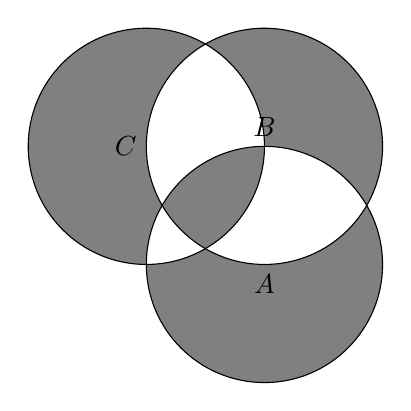
\begin{tikzpicture}
      % Define circles for A, B, and C
      \def\circleA{(0,0) circle (1.5cm)}
      \def\circleB{(1.5,0) circle (1.5cm)}
      \def\circleC{(1.5,-1.5) circle (1.5cm)}

      % Shade for A excluding (B \ C) and (C \ B)
      \begin{scope}
        \clip \circleA;
        \fill[gray] \circleA;
        \clip \circleB;
        \fill[white] \circleB;
      \end{scope}
      
      % Fill the symmetric difference of B and C
      \begin{scope}
        \clip \circleB \circleC; % Start with B and C
        \fill[gray] \circleB \circleC; % Fill B and C
        \clip \circleA; % Remove parts that overlap with A
        \fill[white] \circleA;
      \end{scope}
    
      \begin{scope}
        \clip \circleB;
        \clip \circleC;
        \fill[white] \circleC;
      \end{scope}
    
      \begin{scope}
        \clip \circleC;
        \clip \circleB;
        \fill[white] \circleB;
      \end{scope}

      % Shade the intersection of A, B, and C with a different color
      \begin{scope}
        \clip \circleA;
        \clip \circleB;
        \clip \circleC;
        \fill[gray] \circleC;
      \end{scope}
      
      % Outline the circles and label them
      \draw \circleA node [text=black, left] {$C$};
      \draw \circleB node [text=black, above] {$B$};
      \draw \circleC node [text=black, below] {$A$};
    \end{tikzpicture}
\end{itemize}

We note that we get the same diagram in both cases. Thus proving that the associative law holds.
\pagebreak